\documentclass[11pt]{article}
\usepackage[T1]{fontenc}
\usepackage{textcomp}
\usepackage{lmodern}
\usepackage[margin=1in]{geometry}
\usepackage[pdftex]{graphicx, color}
\usepackage{mathtools}
\usepackage{listings}
\usepackage[pdfusetitle]{hyperref}

\usepackage{tikz}
\usetikzlibrary{automata,positioning}

\renewcommand{\epsilon}{\varepsilon}
\newcommand{\tikzname}{Ti\emph{k}Z}
\tikzset{shorten >=1pt, node distance=2cm, on grid, baseline={([yshift=-8pt] current bounding box.north)}}


\lstset{basicstyle=\small\ttfamily,breaklines=true}

\title{CS143 Spring 2024 -- Written Assignment 1}

\begin{document}
\begin{center}
% Change this:
{\LARGE{CS143 Spring 2024 -- Written Assignment 1}} \\
{\large Due Thursday, April 18, 2024 11:59 PM PDT}
\end{center}

This assignment covers regular languages, finite automata, and lexical analysis. You may discuss this assignment with other students and work on the problems together. However, your write-up should be your own individual work, and you should indicate in your submission who you worked with, if applicable. Assignments can be submitted electronically through Gradescope as a \textsc{pdf} by 11:59 \textsc{pm pdt} on the due date. Please review the course policies for more information: \url{http://web.stanford.edu/class/cs143/policies/index.html}. A \LaTeX{} template for writing your solutions is available on the course website. To create finite automata diagrams, you can either use the \tikzname{} package directly by following the examples in the template, or a tool like \url{https://madebyevan.com/fsm/}.

\begin{enumerate}
% problem 1
\item Write regular expressions for the following languages over the alphabet $\Sigma = \{0, 1\}$.
\begin{enumerate}
    \item The set of strings beginning with 0 and having an odd numbered length.

    \textbf{Solution:}

    \item The set of all strings that contain less than three 1's.

    \textbf{Solution:} 

    \item The set of strings where 0's and 1's appear only in alternating groups of odd numbered length. Examples of strings in the language: $\epsilon$, \underline{0},  \underline{0}\,\underline{111}, \underline{000}\,\underline{1}\,\underline{000}, and \underline{1}\,\underline{0}\,\underline{1}\,\underline{000}. Examples of strings not in the language: 11000, 111011, and 00.

    \textbf{Solution:} 
    
\end{enumerate}

\newpage

% problem 2
\item Draw DFAs for each of the languages from question~1. Note that a DFA must have a transition defined for every state and symbol pair. You must take this fact into account for your transformations. Your DFAs should not have more than 10 states. Submissions with unnecessarily complex DFAs may not receive full credit.

Notice that a short regular expression does not automatically imply a DFA with few states, nor vice versa.

\begin{enumerate}
    \item The set of strings beginning with 0 and having an odd numbered length.\\
    \textbf{Solution:}

    \item The set of all strings that contain less than three 1's.\\
    \textbf{Solution:}

    \item The set of strings where 0's and 1's appear in alternating groups of odd numbered length.\\
    \textbf{Solution:}
    
    
\end{enumerate}

\newpage

% Problem 3
\item Using the techniques covered in class, transform the following NFAs over the alphabet $\{a, b, c\}$ into DFAs. Your DFAs should not have more than 10 states.  Note that a DFA must have a transition defined for every state and symbol pair, whereas a NFA need not. You must take this fact into account for your transformations. Hint: Is there a subset of states the NFA transitions to when fed a symbol for which the set of current states has no explicit transition?

Also include a mapping from each state of your DFA to the corresponding states of the original NFA.  Specifically, a state $q$ of your DFA maps to the set of states $Q$ of the NFA such that an input string stops at $q$ in the DFA if and only if it stops at one of the states in $Q$ in the NFA.

Tip: for readability, states in the DFA may be labeled according to the set of states they represent in the NFA.  For example, state $q_{012}$ in the DFA would correspond to the set of states $\{q_0, q_1, q_2\}$ in the NFA, whereas state $q_{13}$ would correspond to set of states $\{q_1, q_3\}$ in the NFA.

\begin{enumerate}
    \item 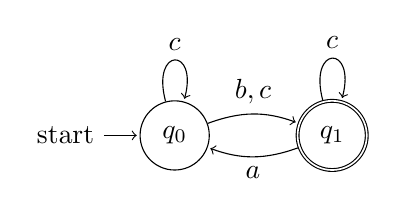
\begin{tikzpicture}[auto]
        \node[state,initial] (q_0) {$q_0$};
        \node[state,accepting] (q_1) [right of=q_0] {$q_1$};
        \path[->]
            (q_0) edge[loop above]   node {$c$}   (q_0)
            (q_0) edge[bend left=20] node {$b,c$} (q_1)
            (q_1) edge[bend left=20] node {$a$}   (q_0)
            (q_1) edge[loop above]   node {$c$}   (q_1);
    \end{tikzpicture}

    \textbf{Solution:}
    
    \item 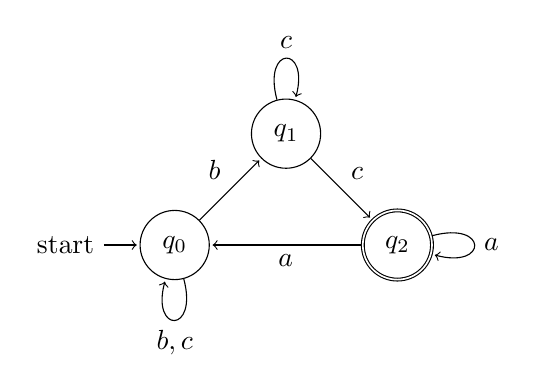
\begin{tikzpicture}[auto]
        \node[state,initial]   (q_0)                      {$q_0$};
        \node[state]           (q_1) [above right of=q_0] {$q_1$};
        \node[state,accepting] (q_2) [below right of=q_1] {$q_2$};
        \path[->]
            (q_0) edge[loop below] node {$b,c$} (q_0)
                  edge             node {$b$}   (q_1)
            (q_1) edge             node {$c$}   (q_2)
            (q_1) edge[loop above] node {$c$}   (q_1)
            (q_2) edge             node {$a$}   (q_0)
            (q_2) edge[loop right] node {$a$}   (q_2);
    \end{tikzpicture}

    \textbf{Solution:}
    
    \item 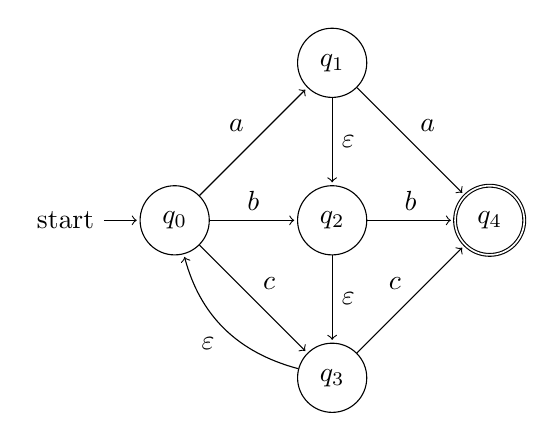
\begin{tikzpicture}[auto]
        \node[state, initial] (q_0) {$q_0$};
        \node[state] (q_2) [right of=q_0] {$q_2$};
        \node[state] (q_3) [below of=q_2] {$q_3$};
        \node[state] (q_1) [above of=q_2] {$q_1$};
        \node[state, accepting] (q_4) [right of=q_2] {$q_4$};

        \path[->]
            (q_0) edge node {$a$} (q_1)
            (q_0) edge node {$b$} (q_2)
            (q_0) edge node {$c$} (q_3)
            (q_1) edge node {$\epsilon$} (q_2)
            (q_2) edge node {$\epsilon$} (q_3)
            (q_3) edge[bend left=30] node {$\epsilon$} (q_0)
            (q_1) edge node {$a$} (q_4)
            (q_2) edge node {$b$} (q_4)
            (q_3) edge node {$c$} (q_4);
        
    \end{tikzpicture}

    \textbf{Solution:}
\end{enumerate}

\newpage

% Problem 4
\item Let $L$ be a language over $\Sigma = \{a, b, c\}$, such that string $w$ is in $L$ if and only if $w\neq\epsilon$ and the last character in $w$ appears an even number of times in $w$

Examples of strings in $L$: $aa$, $abacaba$, $bab$.

Examples of strings \textbf{not} in $L$: $\epsilon$, $a$, $abcabca$, $bbb$.

Draw an NFA for $L$.  Your solution should have no more than 15 states.

\textbf{Solution:}

\newpage

% Problem 5
\item Consider the following tokens and their associated regular expressions, given as a \textbf{flex} scanner specification:
\begin{quote}
\begin{lstlisting}
%%
(01|10)                   printf("apple");
(10)?0?                   printf("banana");
(0110+|1001*1)            printf("coconut");
\end{lstlisting}
\end{quote}
Give an input to this scanner such that the output string is $((\mathtt{apple})^3 (\mathtt{banana})^4)^2 ((\mathtt{apple})^3\mathtt{coconut})^2$, where $\mathtt{A}^i$ denotes $\mathtt{A}$ repeated $i$ times.   (And, of course, the parentheses are not part of the output.)  You may use similar shorthand notation in your answer.

\textbf{Solution:}


\newpage

% Problem 6
\item Recall from the lecture that, when using regular expressions to scan an input, we resolve conflicts by taking the largest possible match at any point. That is, if we have the following \textbf{flex} scanner specification:
\begin{quote}
\begin{lstlisting}
%%
do                      { return T_Do; }
[A-Za-z_][A-Za-z0-9_]*  { return T_Identifier; }
\end{lstlisting}
\end{quote}
and we see the input string ``\texttt{dot}'', we will match the second rule and emit T\_Identifier for the whole string, not T\_Do.

However, it is possible to have a set of regular expressions for which we can tokenize a particular string, but for which taking the largest possible match will fail to break the input into tokens. Give an example of no more than two regular expressions and an input string such that: a) the string can be broken into substrings, where each substring matches one of the regular expressions, b) our usual lexer algorithm, taking the largest match at every step, will fail to break the string in a way in which each piece matches one of the regular expressions. Explain how the string can be tokenized and why taking the largest match won't work in this case.

As a challenge (not necessary for credit), try to find a solution that only uses one regular expression.

\textbf{Solution}:

\end{enumerate}
\end{document}
